\documentclass[]{tufte-book}

% ams
\usepackage{amssymb,amsmath}

\usepackage{ifxetex,ifluatex}
\usepackage{fixltx2e} % provides \textsubscript
\ifnum 0\ifxetex 1\fi\ifluatex 1\fi=0 % if pdftex
  \usepackage[T1]{fontenc}
  \usepackage[utf8]{inputenc}
\else % if luatex or xelatex
  \makeatletter
  \@ifpackageloaded{fontspec}{}{\usepackage{fontspec}}
  \makeatother
  \defaultfontfeatures{Ligatures=TeX,Scale=MatchLowercase}
  \makeatletter
  \@ifpackageloaded{soul}{
     \renewcommand\allcapsspacing[1]{{\addfontfeature{LetterSpace=15}#1}}
     \renewcommand\smallcapsspacing[1]{{\addfontfeature{LetterSpace=10}#1}}
   }{}
  \makeatother

\fi

% graphix
\usepackage{graphicx}
\setkeys{Gin}{width=\linewidth,totalheight=\textheight,keepaspectratio}

% booktabs
\usepackage{booktabs}

% url
\usepackage{url}

% hyperref
\usepackage{hyperref}

% units.
\usepackage{units}


\setcounter{secnumdepth}{2}

% citations


% pandoc syntax highlighting

% table with pandoc
\usepackage{longtable,booktabs,array}
\usepackage{calc} % for calculating minipage widths
% Correct order of tables after \paragraph or \subparagraph
\usepackage{etoolbox}
\makeatletter
\patchcmd\longtable{\par}{\if@noskipsec\mbox{}\fi\par}{}{}
\makeatother
% Allow footnotes in longtable head/foot
\IfFileExists{footnotehyper.sty}{\usepackage{footnotehyper}}{\usepackage{footnote}}
\makesavenoteenv{longtable}

% multiplecol
\usepackage{multicol}

% strikeout
\usepackage[normalem]{ulem}

% morefloats
\usepackage{morefloats}


% tightlist macro required by pandoc >= 1.14
\providecommand{\tightlist}{%
  \setlength{\itemsep}{0pt}\setlength{\parskip}{0pt}}

% title / author / date
\title{Fire science workshop materials}
\author{Devan Allen McGranahan \(*\)\\
~\\
\(*\) USDA-ARS\\}
\date{Version date: 18 February 2022}

\renewcommand\familydefault{\sfdefault}

\begin{document}

\maketitle




\hypertarget{summary}{%
\chapter{Summary}\label{summary}}

Here's a citation (McGranahan
\protect\hyperlink{ref-mcgranahan2021}{2021}).

\hypertarget{findings}{%
\section{Findings}\label{findings}}

\hypertarget{references}{%
\chapter{References}\label{references}}

\hypertarget{headings}{%
\chapter{Headings}\label{headings}}

This style provides first and second-level headings (that is,
\texttt{\#} and \texttt{\#\#}), demonstrated in the next section. You
may get unexpected output if you try to use \texttt{\#\#\#} and smaller
headings.

\newthought{In his later books}\footnote{\href{https://www.edwardtufte.com/tufte/books_be}{Beautiful
  Evidence}}, Tufte starts each section with a bit of vertical space, a
non-indented paragraph, and sets the first few words of the sentence in
small caps. To accomplish this using this style, call the
\texttt{newthought()} function in \textbf{tufte} in an \emph{inline R
expression} \texttt{\textasciigrave{}r\ \textasciigrave{}} as
demonstrated at the beginning of this paragraph.\footnote{Note you
  should not assume \textbf{tufte} has been attached to your R session.
  You should either \texttt{library(tufte)} in your R Markdown document
  before you call \texttt{newthought()}, or use
  \texttt{tint::newthought()}.}

\hypertarget{figures}{%
\chapter{Figures}\label{figures}}

\hypertarget{margin-figures}{%
\section{Margin Figures}\label{margin-figures}}

Images and graphics play an integral role in Tufte's work. To place
figures in the margin you can use the \textbf{knitr} chunk option
\texttt{fig.margin\ =\ TRUE}. For example:

\begin{marginfigure}
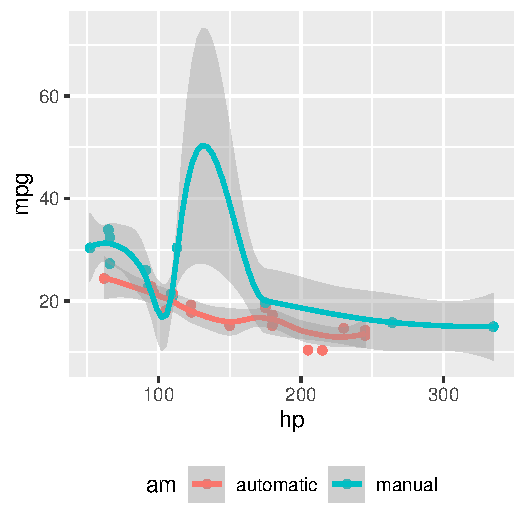
\includegraphics{FireScienceMethodsBook_files/figure-latex/fig-margin-1} \caption[MPG vs horsepower, colored by transmission]{MPG vs horsepower, colored by transmission.}\label{fig:fig-margin}
\end{marginfigure}

Note the use of the \texttt{fig.cap} chunk option to provide a figure
caption. You can adjust the proportions of figures using the
\texttt{fig.width} and \texttt{fig.height} chunk options. These are
specified in inches, and will be automatically scaled down to fit within
the handout margin.

\hypertarget{arbitrary-margin-content}{%
\section{Arbitrary Margin Content}\label{arbitrary-margin-content}}

In fact, you can include anything in the margin using the \textbf{knitr}
engine named \texttt{marginfigure}. Unlike R code chunks
\texttt{\textasciigrave{}\textasciigrave{}\textasciigrave{}\{r\}}, you
write a chunk starting with
\texttt{\textasciigrave{}\textasciigrave{}\textasciigrave{}\{marginfigure\}}
instead, then put the content in the chunk. See an example on the right
about the first fundamental theorem of calculus.

For the sake of portability between LaTeX and HTML, you should keep the
margin content as simple as possible (syntax-wise) in the
\texttt{marginefigure} blocks. You may use simple Markdown syntax like
\texttt{**bold**} and \texttt{\_italic\_} text, but please refrain from
using footnotes, citations, or block-level elements (e.g.~blockquotes
and lists) there.

\hypertarget{full-width-figures}{%
\section{Full Width Figures}\label{full-width-figures}}

You can arrange for figures to span across the entire page by using the
chunk option \texttt{fig.fullwidth\ =\ TRUE}.

\begin{figure*}
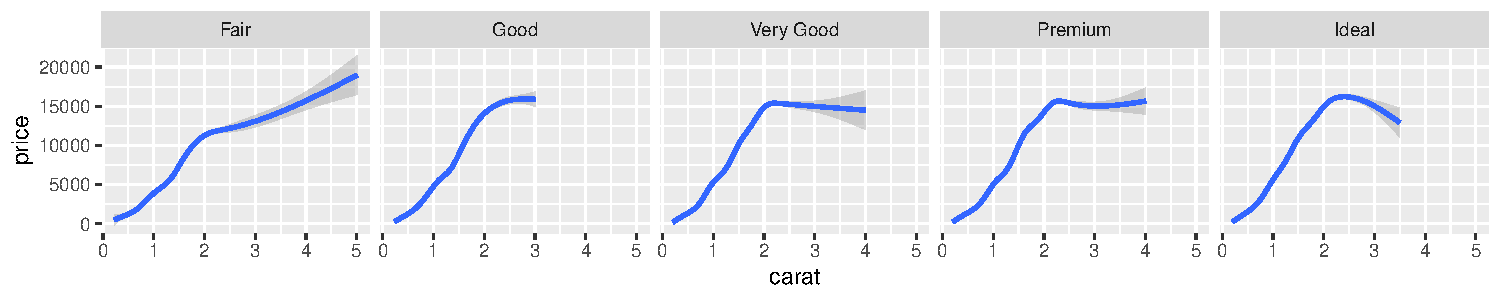
\includegraphics{FireScienceMethodsBook_files/figure-latex/fig-fullwidth-1} \caption[A full width figure]{A full width figure.}\label{fig:fig-fullwidth}
\end{figure*}

Other chunk options related to figures can still be used, such as
\texttt{fig.width}, \texttt{fig.cap}, \texttt{out.width}, and so on. For
full width figures, usually \texttt{fig.width} is large and
\texttt{fig.height} is small. In the above example, the plot size is
\(10 \times 2\).

\hypertarget{main-column-figures}{%
\section{Main Column Figures}\label{main-column-figures}}

Besides margin and full width figures, you can of course also include
figures constrained to the main column. This is the default type of
figures in the LaTeX/HTML output.

\begin{figure}
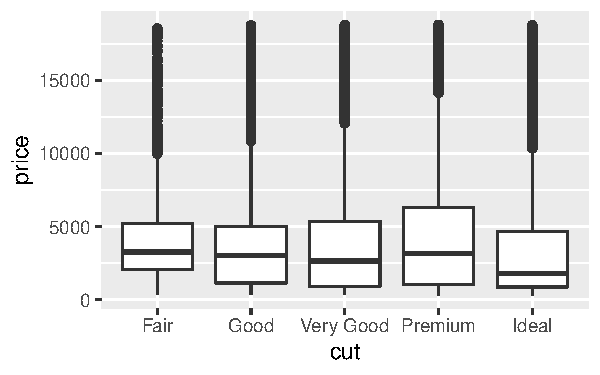
\includegraphics{FireScienceMethodsBook_files/figure-latex/fig-main-1} \caption[A figure in the main column]{A figure in the main column.}\label{fig:fig-main}
\end{figure}

\hypertarget{sidenotes}{%
\chapter{Sidenotes}\label{sidenotes}}

One of the most prominent and distinctive features of this style is the
extensive use of sidenotes. There is a wide margin to provide ample room
for sidenotes and small figures. Any use of a footnote will
automatically be converted to a sidenote.\footnote{This is a sidenote
  that was entered using a footnote.}

If you'd like to place ancillary information in the margin without the
sidenote mark (the superscript number), you can use the
\texttt{margin\_note()} function from \textbf{tufte} in an inline R
expression.
\marginnote{This is a margin note.  Notice that there is no number preceding the note.}
This function does not process the text with Pandoc, so Markdown syntax
will not work here. If you need to write anything in Markdown syntax,
please use the \texttt{marginfigure} block described previously.

\hypertarget{references-1}{%
\chapter{References}\label{references-1}}

References can be displayed as margin notes for HTML output. For
example, we can cite a paper here (McGranahan
\protect\hyperlink{ref-mcgranahan2021}{2021}).

\hypertarget{tables}{%
\chapter{Tables}\label{tables}}

You can use the \texttt{kable()} function from the \textbf{knitr}
package to format tables that integrate well with the rest of the Tufte
handout style. The table captions are placed in the margin like figures
in the HTML output.

\begin{longtable}[]{@{}lrrrrrr@{}}
\caption{A subset of mtcars.}\tabularnewline
\toprule
& mpg & cyl & disp & hp & drat & wt\tabularnewline
\midrule
\endfirsthead
\toprule
& mpg & cyl & disp & hp & drat & wt\tabularnewline
\midrule
\endhead
Mazda RX4 & 21.0 & 6 & 160 & 110 & 3.90 & 2.620\tabularnewline
Mazda RX4 Wag & 21.0 & 6 & 160 & 110 & 3.90 & 2.875\tabularnewline
Datsun 710 & 22.8 & 4 & 108 & 93 & 3.85 & 2.320\tabularnewline
Hornet 4 Drive & 21.4 & 6 & 258 & 110 & 3.08 & 3.215\tabularnewline
Hornet Sportabout & 18.7 & 8 & 360 & 175 & 3.15 & 3.440\tabularnewline
Valiant & 18.1 & 6 & 225 & 105 & 2.76 & 3.460\tabularnewline
\bottomrule
\end{longtable}

\hypertarget{block-quotes}{%
\chapter{Block Quotes}\label{block-quotes}}

We know from the Markdown syntax that paragraphs that start with
\texttt{\textgreater{}} are converted to block quotes. If you want to
add a right-aligned footer for the quote, you may use the function
\texttt{quote\_footer()} from \textbf{tufte} in an inline R expression.
Here is an example:

\begin{quote}
``If it weren't for my lawyer, I'd still be in prison. It went a lot
faster with two people digging.''

\hfill --- Joe Martin
\end{quote}

Without using \texttt{quote\_footer()}, it looks like this (the second
line is just a normal paragraph):

\begin{quote}
``Great people talk about ideas, average people talk about things, and
small people talk about wine.''

--- Fran Lebowitz
\end{quote}

\hypertarget{some-notes-on-tufte-css}{%
\chapter{Some Notes on Tufte CSS}\label{some-notes-on-tufte-css}}

There are a few other things in Tufte CSS that we have not mentioned so
far. If you prefer \textsf{sans-serif fonts}, use the function
\texttt{sans\_serif()} in \textbf{tufte}. For epigraphs, you may use a
pair of underscores to make the paragraph italic in a block quote, e.g.

\begin{quote}
\emph{I can win an argument on any topic, against any opponent. People
know this, and steer clear of me at parties. Often, as a sign of their
great respect, they don't even invite me.}

\hfill --- Dave Barry
\end{quote}

\hypertarget{references-2}{%
\chapter*{References}\label{references-2}}
\addcontentsline{toc}{chapter}{References}

\hypertarget{refs}{}
\leavevmode\hypertarget{ref-mcgranahan2021}{}%
McGranahan DA (2021) FeatherFlame: An Arduino-based thermocouple
datalogging system to record wildland fire flame temperatures \emph{in
agris}. \emph{Rangeland Ecology and Management} \textbf{76}, 43--47.
doi:\href{https://doi.org/https://doi.org/10.1016/j.rama.2021.01.008}{https://doi.org/10.1016/j.rama.2021.01.008}.



\end{document}
